\chapter{Τεχνολογιές}

\section{Εισαγωγή}

Αρχικά δημιουργήθηκε η βασική δομή και η δομή της διαδικτυακής πύλης καθορίστηκε. Αυτή η βασική δομή φαίνεται στο Παρακάτω σχήμα

Είναι σημαντικό να σημειωθεί ότι ολόκληρη η εφαρμογή Django βρίσκεται στον ίδιο φυσικό
διακομιστή. Όταν ο χρήστης στέλνει ένα αίτημα για την εκτέλεση ενός σεναρίου με συγκεκριμένες εισόδους αυτό στέλνεται στις συσκευές στο τοπικό δίκτυο.


Το πρώτο βήμα στη διαδικασία ήταν να καθοριστεί τι θα αυτοματοποιηθεί με βάση τις
διάφορες εκτιμήσεις. Για να καθοριστεί αυτό, πραγματοποιήθηκαν πολλές συναντήσεις καταιγισμού ιδεών.
με την ομάδα. Προτού γίνει αυτό όμως η αρχική ιδεά που τέθηκε στο τραπέζι βγήκε με βάση μια παρόμοια δουλειά ενός μηχανικού
της \en{Cisco}. Το έργο του θα αναφερθεί αναλυτικά στην εκτενή βιβλιογραφία στο τέλος. Με βάση λοιπόν
αυτο το έργο ξεκινήσαν συζητήσεις για το πως θα μπορέσουμε να αναπτύξουμε κάτι παρόμοιο
καθώς και να το εμπλουτίσουμε στο τέλος έτσι ώστε να αντοπρίνεται όσο γίνεται στις τεχνολογίες του
σήμερα.

Σε αυτές τις συναντήσεις που γίνανε μεταξύ μας τέθηκαν πολλές ιδέες τέθηκαν στο τραπέζι και η ομάδα καθόρισε
μια σειρά προτεραιότητας για την ανάπτυξη. Ο στόχος σε πολλούς αυτοματισμούς είναι να μειωθεί ο χρόνος που καταναλώνεται για την εκτέλεση
αυτές τις επαναλαμβανόμενες εργασίες. Πολλές τεχνολογίες χρησιμοποιήθηκαν για την υλοποίηση του συγκεκριμένου έργου οι οποίες θα παρουσιαστούν
εκτενώς σε άλλες ενότητες.

Η υλοποίησή μιας τέτοιας εφαρμογής είχε κάποιες δυσκολίες. Κυρίως ποιο θα είναι το περιβάλλον στο οποίο
η εφαρμογή θα μπορούσε να τεσταριστεί και υλοποιηθεί. Για αυτό πάρθηκε η απόφαση οι συσκευές με τις οποίες θα τεσταριστεί
και συνάμα θα λειτουργήσει η εφαρμογή θα είναι \en{virtual }συσκευές της \en{Cisco} οι οποίες θα τρέχουν στο \en{GNS3}
και το \en{GNS3} θα μπορεί να επικοινωνεί δικτυακά με τον \en{Django Server} στο τοπικό δίκτυο.
Το στήσιμο όλου του περιβάλλοντος και της εφαρμογής θα αναλυθεί εκτενώς περαιτέρω σε άλλο κεφάλαιο.


\section{\en{GNS3}}
Το \en{GNS3} Είναι ένα εργαλείο προσομοίωσης δικτύων ανοικτού κώδικα που επιτρέπει στους χρήστες να προσομοιώσουν 
σύνθετες τοπολογίες δικτύων στους υπολογιστές τους. Μηχανικοί δικτύων και φοιτητές 
το χρησιμοποιούν ευρέως για να μάθουν και να εξασκηθούν σε έννοιες δικτύωσης, να δοκιμάσουν διαμορφώσεις δικτύου και να δημιουργήσουν εικονικά περιβάλλοντα δικτύου.


Το \en{GNS3} υποστηρίζει διάφορες συσκευές δικτύου, όπως δρομολογητές, μεταγωγείς και τείχη προστασίας 
από διάφορους προμηθευτές, συμπεριλαμβανομένων των \en{Cisco}, \en{Juniper}, \en{Nokia} και άλλων. Επιτρέπει στους χρήστες να 
προσομοιώσουν διάφορα σενάρια και διαμορφώσεις δικτύου και να δοκιμάσουν τη συμπεριφορά των 
συσκευών δικτύου σε ένα ελεγχόμενο περιβάλλον. 

\begin{figure}[htb]
	\centering
	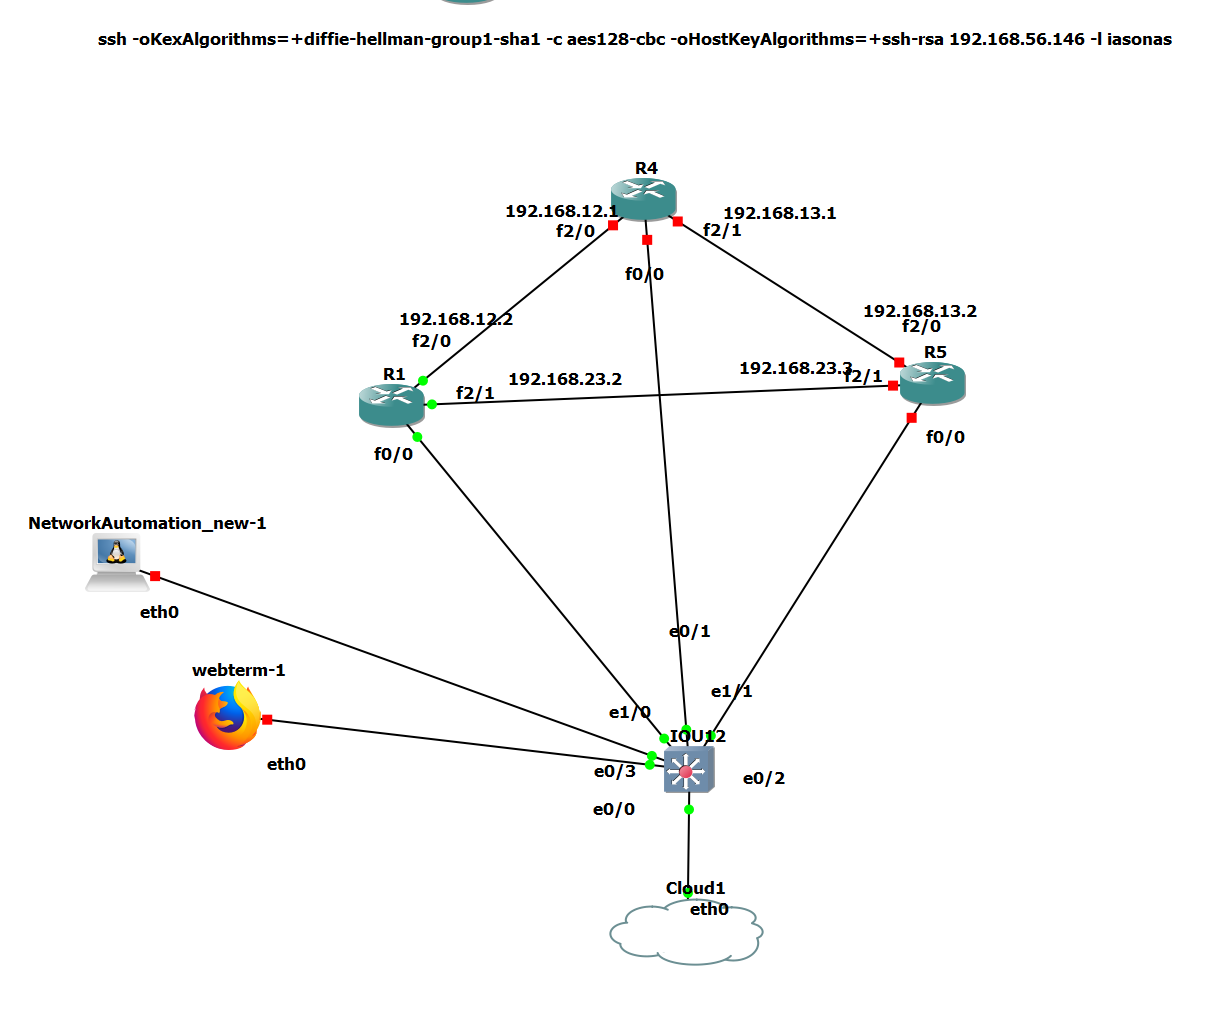
\includegraphics[width=0.7\textwidth]{graphics/Network_topology.png}
	\caption{\en{General Network Topology} }
\end{figure}



\section{\en{Cisco IOS}}
Το \en{IOU} σημαίνει \en{IOS on Unix} είναι μια εικονική έκδοση του λογισμικού \en{IOS} της \en{Cisco} που 
μπορεί να χρησιμοποιηθεί για σκοπούς προσομοίωσης και δοκιμής δικτύου. Επιτρέπει στους μηχανικούς δικτύου να δημιουργούν εικονικές τοπολογίες δικτύου και να εξασκούνται σε διάφορες εργασίες δικτύου, 
όπως η διαμόρφωση δρομολογητών και μεταγωγέων, χωρίς να απαιτείται φυσικό υλικό. Το πλεονέκτημα του \en{GNS3} σε σχέση με εφαρμογές άλλες όπως το \en{Packet tracer} είναι ότι το \en{GNS3} 
μπορεί να σηκώσει πραγματικά \en{images} άρα πραγματικό λογισμικό συνεπώς οι λειτουργίες που μπορείς να κάνεις είναι πολύ περισσότερες.

Το \en{Cisco IOU} χρησιμοποιείται συχνά σε συνδυασμό με λογισμικό προσομοίωσης δικτύου όπως 
\en{GNS3} ή \en{EVE-NG}, τα οποία αποτελούν την πλατφόρμα εικονικοποίησης δικτύου που σας επιτρέπει να 
να δημιουργείτε και να διαχειρίζεστε εικονικά περιβάλλοντα δικτύου για σκοπούς δοκιμής και εκμάθησης, τα οποία παρέχουν ένα γραφικό περιβάλλον χρήστη για τη δημιουργία και τη διαχείριση εικονικών 
τοπολογιών δικτύου. Οι εικόνες \en{IOU} μπορούν να φορτωθούν σε αυτά τα εργαλεία προσομοίωσης για τη δημιουργία εικονικών συσκευών \en{Cisco} που μπορούν να διαμορφωθούν και να δοκιμαστούν όπως το φυσικό δίκτυο 
συσκευές.

\section{Εικονικοποίηση}
Στην επιστήμη της πληροφορικής, η εικονικοποίηση \en{virtualization} είναι ένας ευρύς όρος 
των υπολογιστικών συστημάτων που αναφέρεται σε έναν μηχανισμό αφαίρεσης, 
στοχευμένο στην απόκρυψη λεπτομερειών της υλοποίησης και της κατάστασης
ορισμένων υπολογιστικών πόρων από πελάτες των πόρων αυτών 
(π.χ. εφαρμογές, άλλα συστήματα, χρήστες κλπ). 
Η εν λόγω αφαίρεση μπορεί είτε να αναγκάζει έναν πόρο να 
συμπεριφέρεται ως πλειάδα πόρων (π.χ. μία συσκευή αποθήκευσης σε διακομιστή τοπικού δικτύου),
είτε πολλαπλούς πόρους να συμπεριφέρονται ως ένας (π.χ. συσκευές αποθήκευσης σε κατανεμημένα συστήματα). 

Η εικονικοποίηση δημιουργεί μία εξωτερική διασύνδεση η οποία αποκρύπτει την 
υποκείμενη υλοποίηση (π.χ. πολυπλέκοντας την πρόσβαση από διαφορετικούς χρήστες).
Αυτή η προσέγγιση στην εικονικοποίηση αναφέρεται ως εικονικοποίηση πόρων. 
Μία άλλη προσέγγιση, ίδιας όμως νοοτροπίας, είναι η εικονικοποίηση πλατφόρμας,
όπου η αφαίρεση που επιτελείται προσομοιώνει ολόκληρους υπολογιστές. Το αντίθετο της εικονικοποίησης είναι η διαφάνεια: 
ένας εικονικός πόρος είναι ορατός, αντιληπτός, αλλά στην πραγματικότητα ανύπαρκτος, 
ενώ ένας διαφανής πόρος είναι υπαρκτός αλλά αόρατος. 
 
Θα εξηγήσουμε την εικονικοποίηση στην δικιά μας περίπτωση. Το πρώτο επίπεδο είναι αυτό του υλικού. Η εικονικοποίηση
σα τεχνολογία εικονοποιεί το υλικό για να μπορέσει να δώσε πόρους στις εικονικές μηχανές. Η υλοιποίηση
της εικονικοποίησης γίνεται με λογισμικό \en{hypervisor}. Στη δικιά μας περίπτωση ο \en{hypervisor} είναι 
το \en{Virtual Box} ο οποίος είναι ένας τύπου Β \en{hypervisor}. Ο \en{hypervisor} τύπου 2 είναι μια εφαρμογή εγκατεστημένη 
στο λειτουργικό σύστημα του κεντρικού υπολογιστή το οποίο μας δίνει τη δυνατότητα να σηκώσουμε 
εικονικές μηχανές άλλων λειτουργικών συστημάτων πάνω στο ήδη υπάρχον σύστημα.

Οι παρακάτω εικόνες μπορούν να εξηγήσουν σχηματικά τη γενική καθώς και την ειδική αρχιτεκτονική.

\begin{figure}[htb]
	\centering
	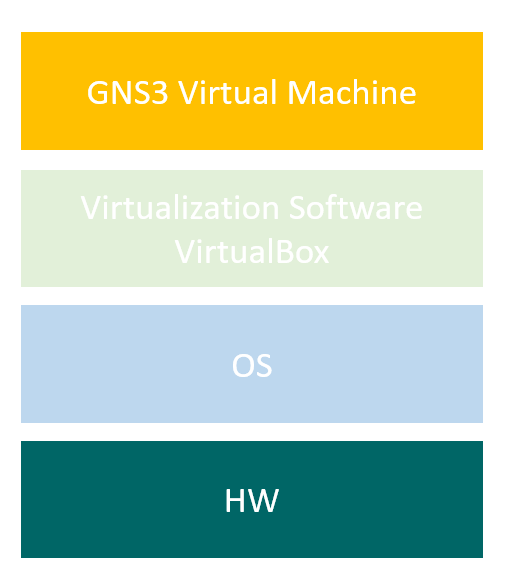
\includegraphics[width=0.5\textwidth]{graphics/Architecture_virtualbox.PNG}
	\caption{\en{Virtualization} Γενική αρχιτεκτονική}
\end{figure}

\begin{figure}[htb]
	\centering
	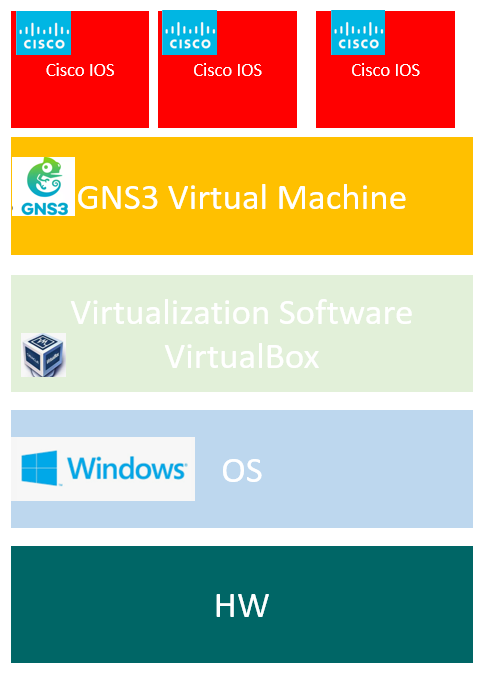
\includegraphics[width=0.5\textwidth]{graphics/virtualization_architecture.PNG}
	\caption{\en{Virtualization} Γενική αρχιτεκτονική}
\end{figure}








